\documentclass[11pt,a4paper]{article}
\usepackage{graphicx}
\usepackage{subfigure}
\usepackage{amsmath}
\usepackage{makecell}
\usepackage[utf8]{inputenc}
\usepackage{listings} %放代码
\usepackage{xcolor} %代码着色宏包
\usepackage{color} %代码着色宏包
\usepackage{xeCJK}
\usepackage{float}

%好像是数学的包
\usepackage{amsmath}
\usepackage{amssymb}
\usepackage{mathrsfs}
%页面布局包
\usepackage{geometry}
%画图包
\usepackage{tikz}
%画图背景包
\usetikzlibrary{backgrounds}

\geometry{left=3.0cm, right=3.0cm, top=3cm, bottom=3cm}

%自定义命令
\newcommand{\psiG}{\psi_{G}}
%在tikz中画一个顶点
%#1:node名称
%#2:位置
%#3:标签
\newcommand{\newVertex}[3]{\node[circle, draw=black, line width=1pt, scale=0.8] (#1) at #2{#3}}
%在tikz中画一条边
\newcommand{\newEdge}[2]{\draw [black,very thick](#1)--(#2)}
%在tikz中放一个标签
%#1:名称
%#2:位置
%#3:标签内容
\newcommand{\newLabel}[3]{\node[line width=1pt] (#1) at #2{#3}}


\title{Introduction to Computing Systems\\Homework 2}
\author{PB18111697 王章瀚}

\begin{document}
	\maketitle
	\section{}
	\subsection*{a}
	\begin{figure}[H]
		\centering
		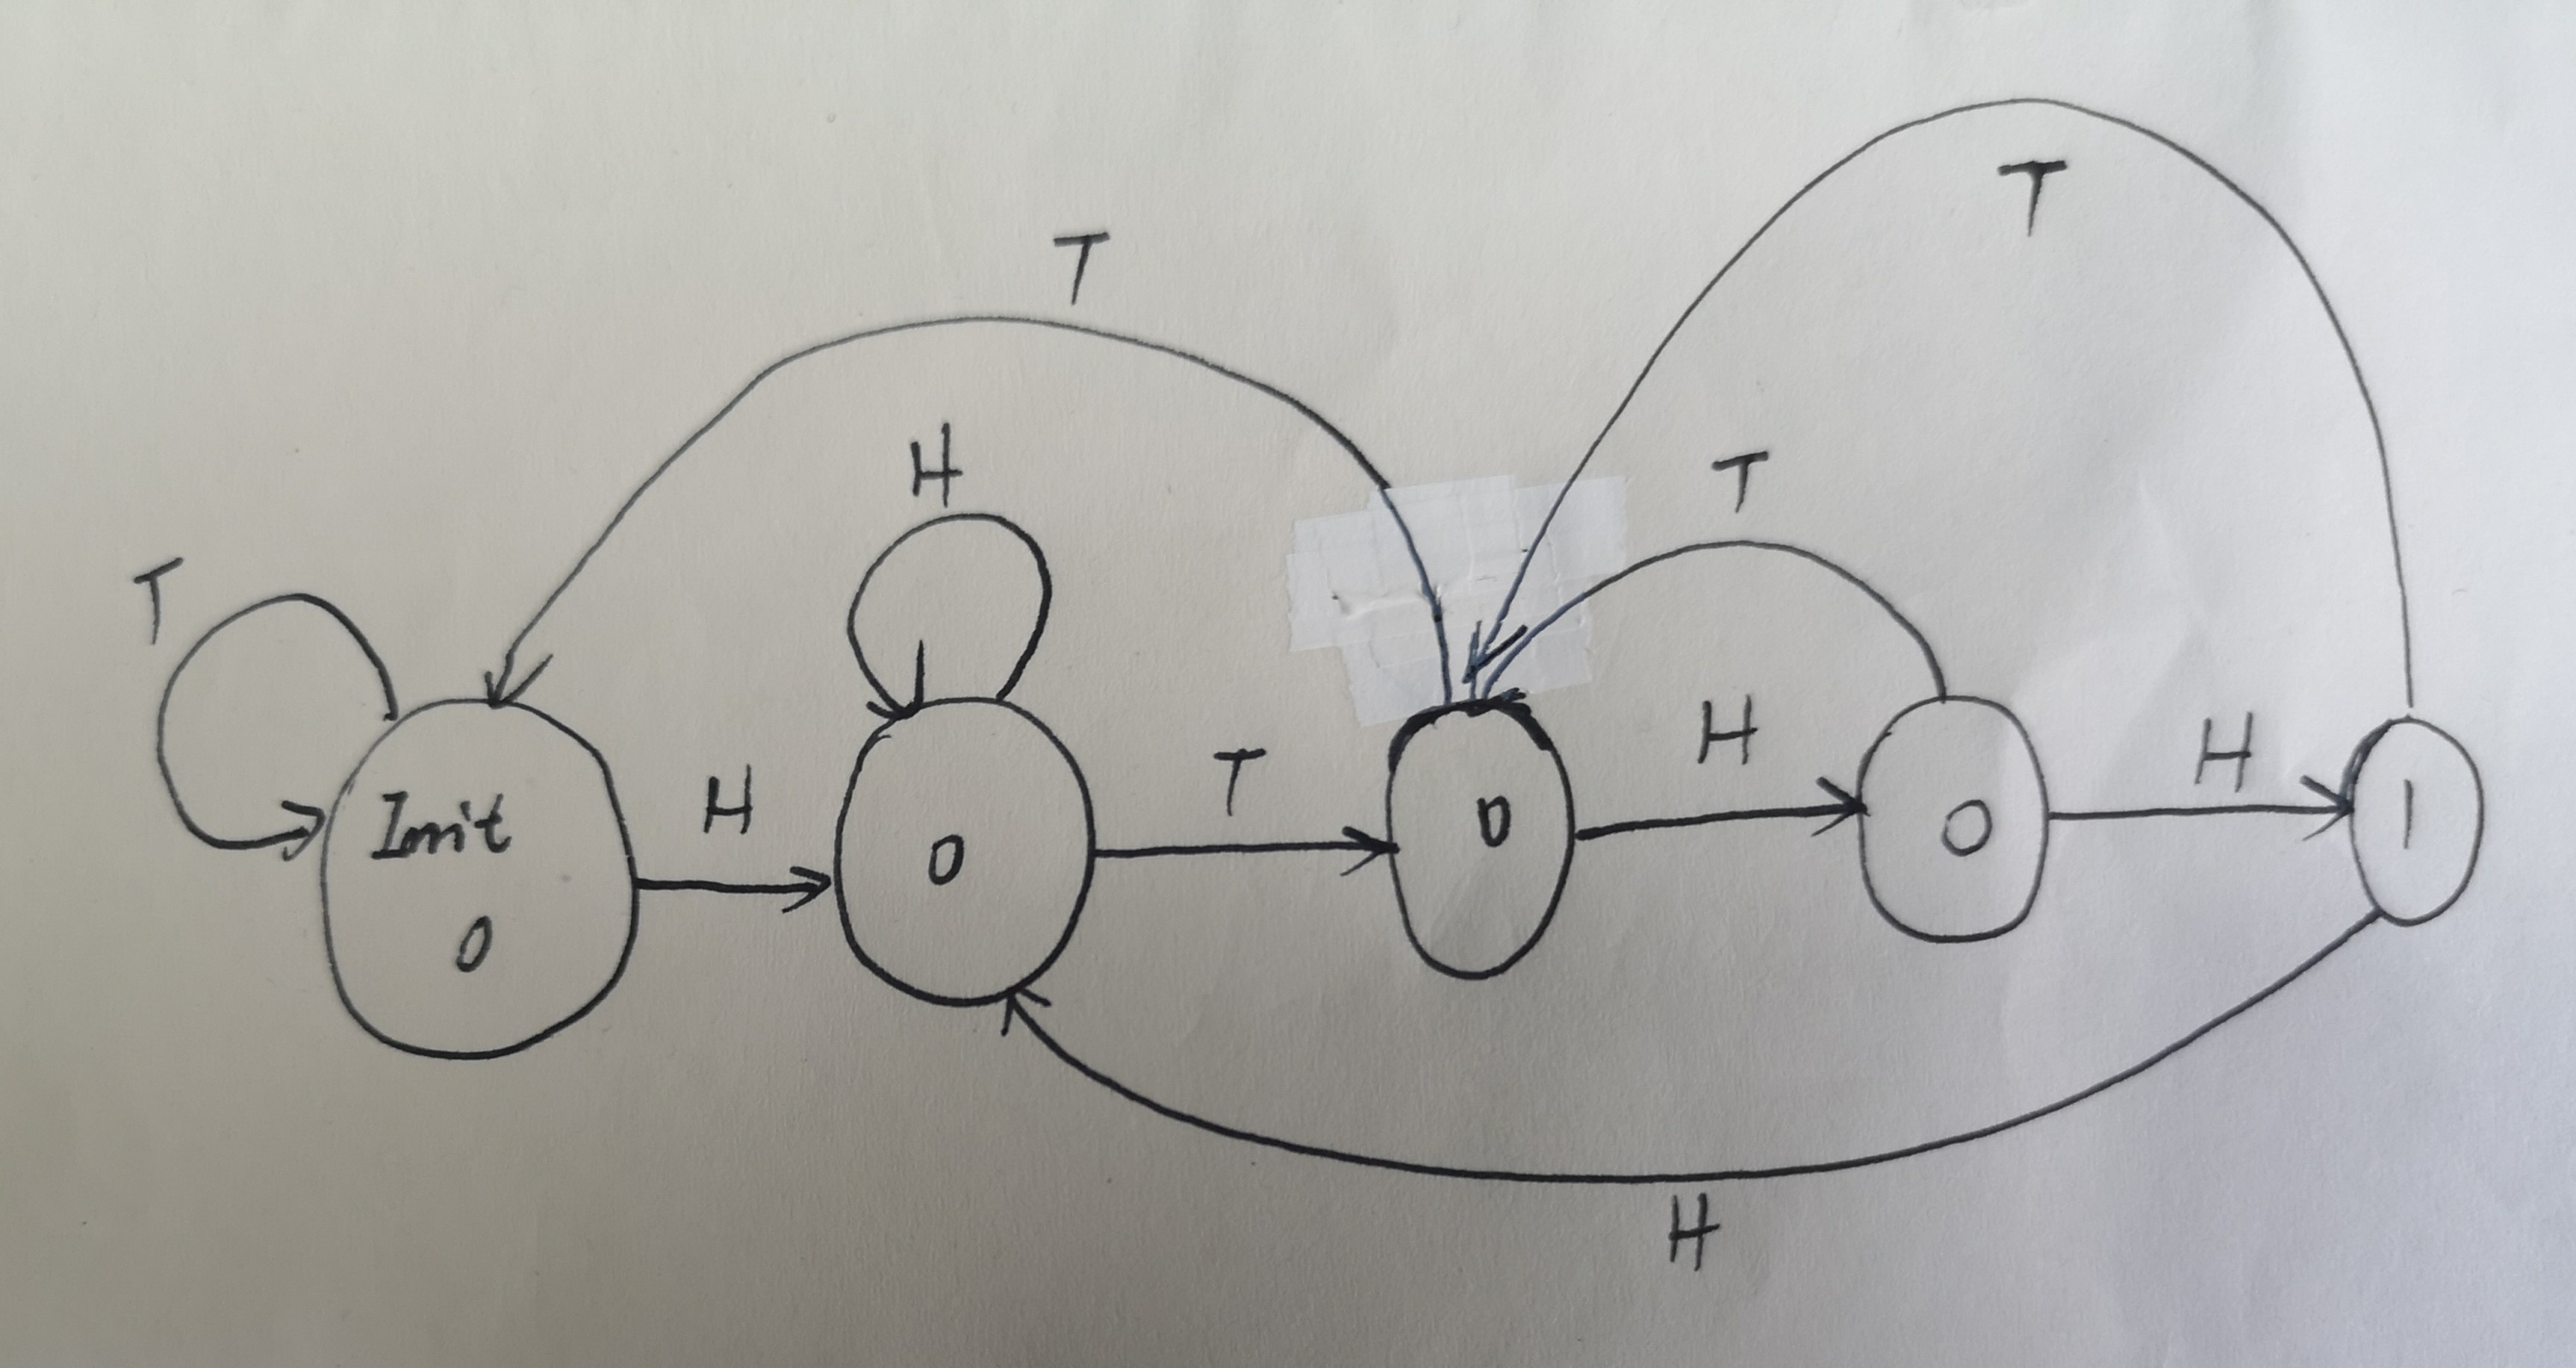
\includegraphics[width=1\linewidth]{1_a.jpg}
		\label{1_a}
	\end{figure}
	\subsection*{b}
	Since there are 5 states in all, \underline{3 state variables(I mean a variables with 3 bits)} will be needed.
	
	\section{}
	The addressability is 16 byte and it has $2^{7}$ memory locations, so the computer has \underline{$16byte\times 2^{7}=2048$} bytes of memory.
	
	
	\section{}
	\subsection*{a \textcolor{red}{"A[1:0] should be 01", pat attention to the circuit.}}
	A[1:0]=10, WE = 1
	\subsection*{b}
	It needs $\lceil log_2(800)\rceil=10$ address lines.\\
	And the addressability maintains.
	\subsection*{c}
	$2^{10}-\lceil log_2(800)\rceil=\underline{224}$
	
	\section{}
	\subsection*{a}
	The address space of this memory is \underline{2 bits}, which is $2^{2}=\underline{4}$ locations.
	\subsection*{b}
	The addressability of this memory is \underline{16 bits}.
	\subsection*{c}
	It's $4\times 16\ bits=\underline{8\ bytes}$
	\subsection*{d}
	\begin{tabular}{|c|c|c|c|c|}
		\hline 
		WE & A[1:0] & Di[15:0] & D[15:0] & Read/Write \\ 
		\hline 
		0 & 01 & xFADE & \underline{x4567} & \underline{Read} \\ 
		\hline 
		1 & 10 & xDEAD & \underline{xDEAD} & \underline{Write} \\ 
		\hline 
		\underline{0} & \underline{00} & xBEEF & x0123 & Read \\ 
		\hline 
		\underline{1} & 11 & \underline{xFEED} & xFEED & Write \\ 
		\hline 
	\end{tabular} 
	
	\section{}
	And the states diagram is as below.
	\begin{figure}[H]
		\centering
		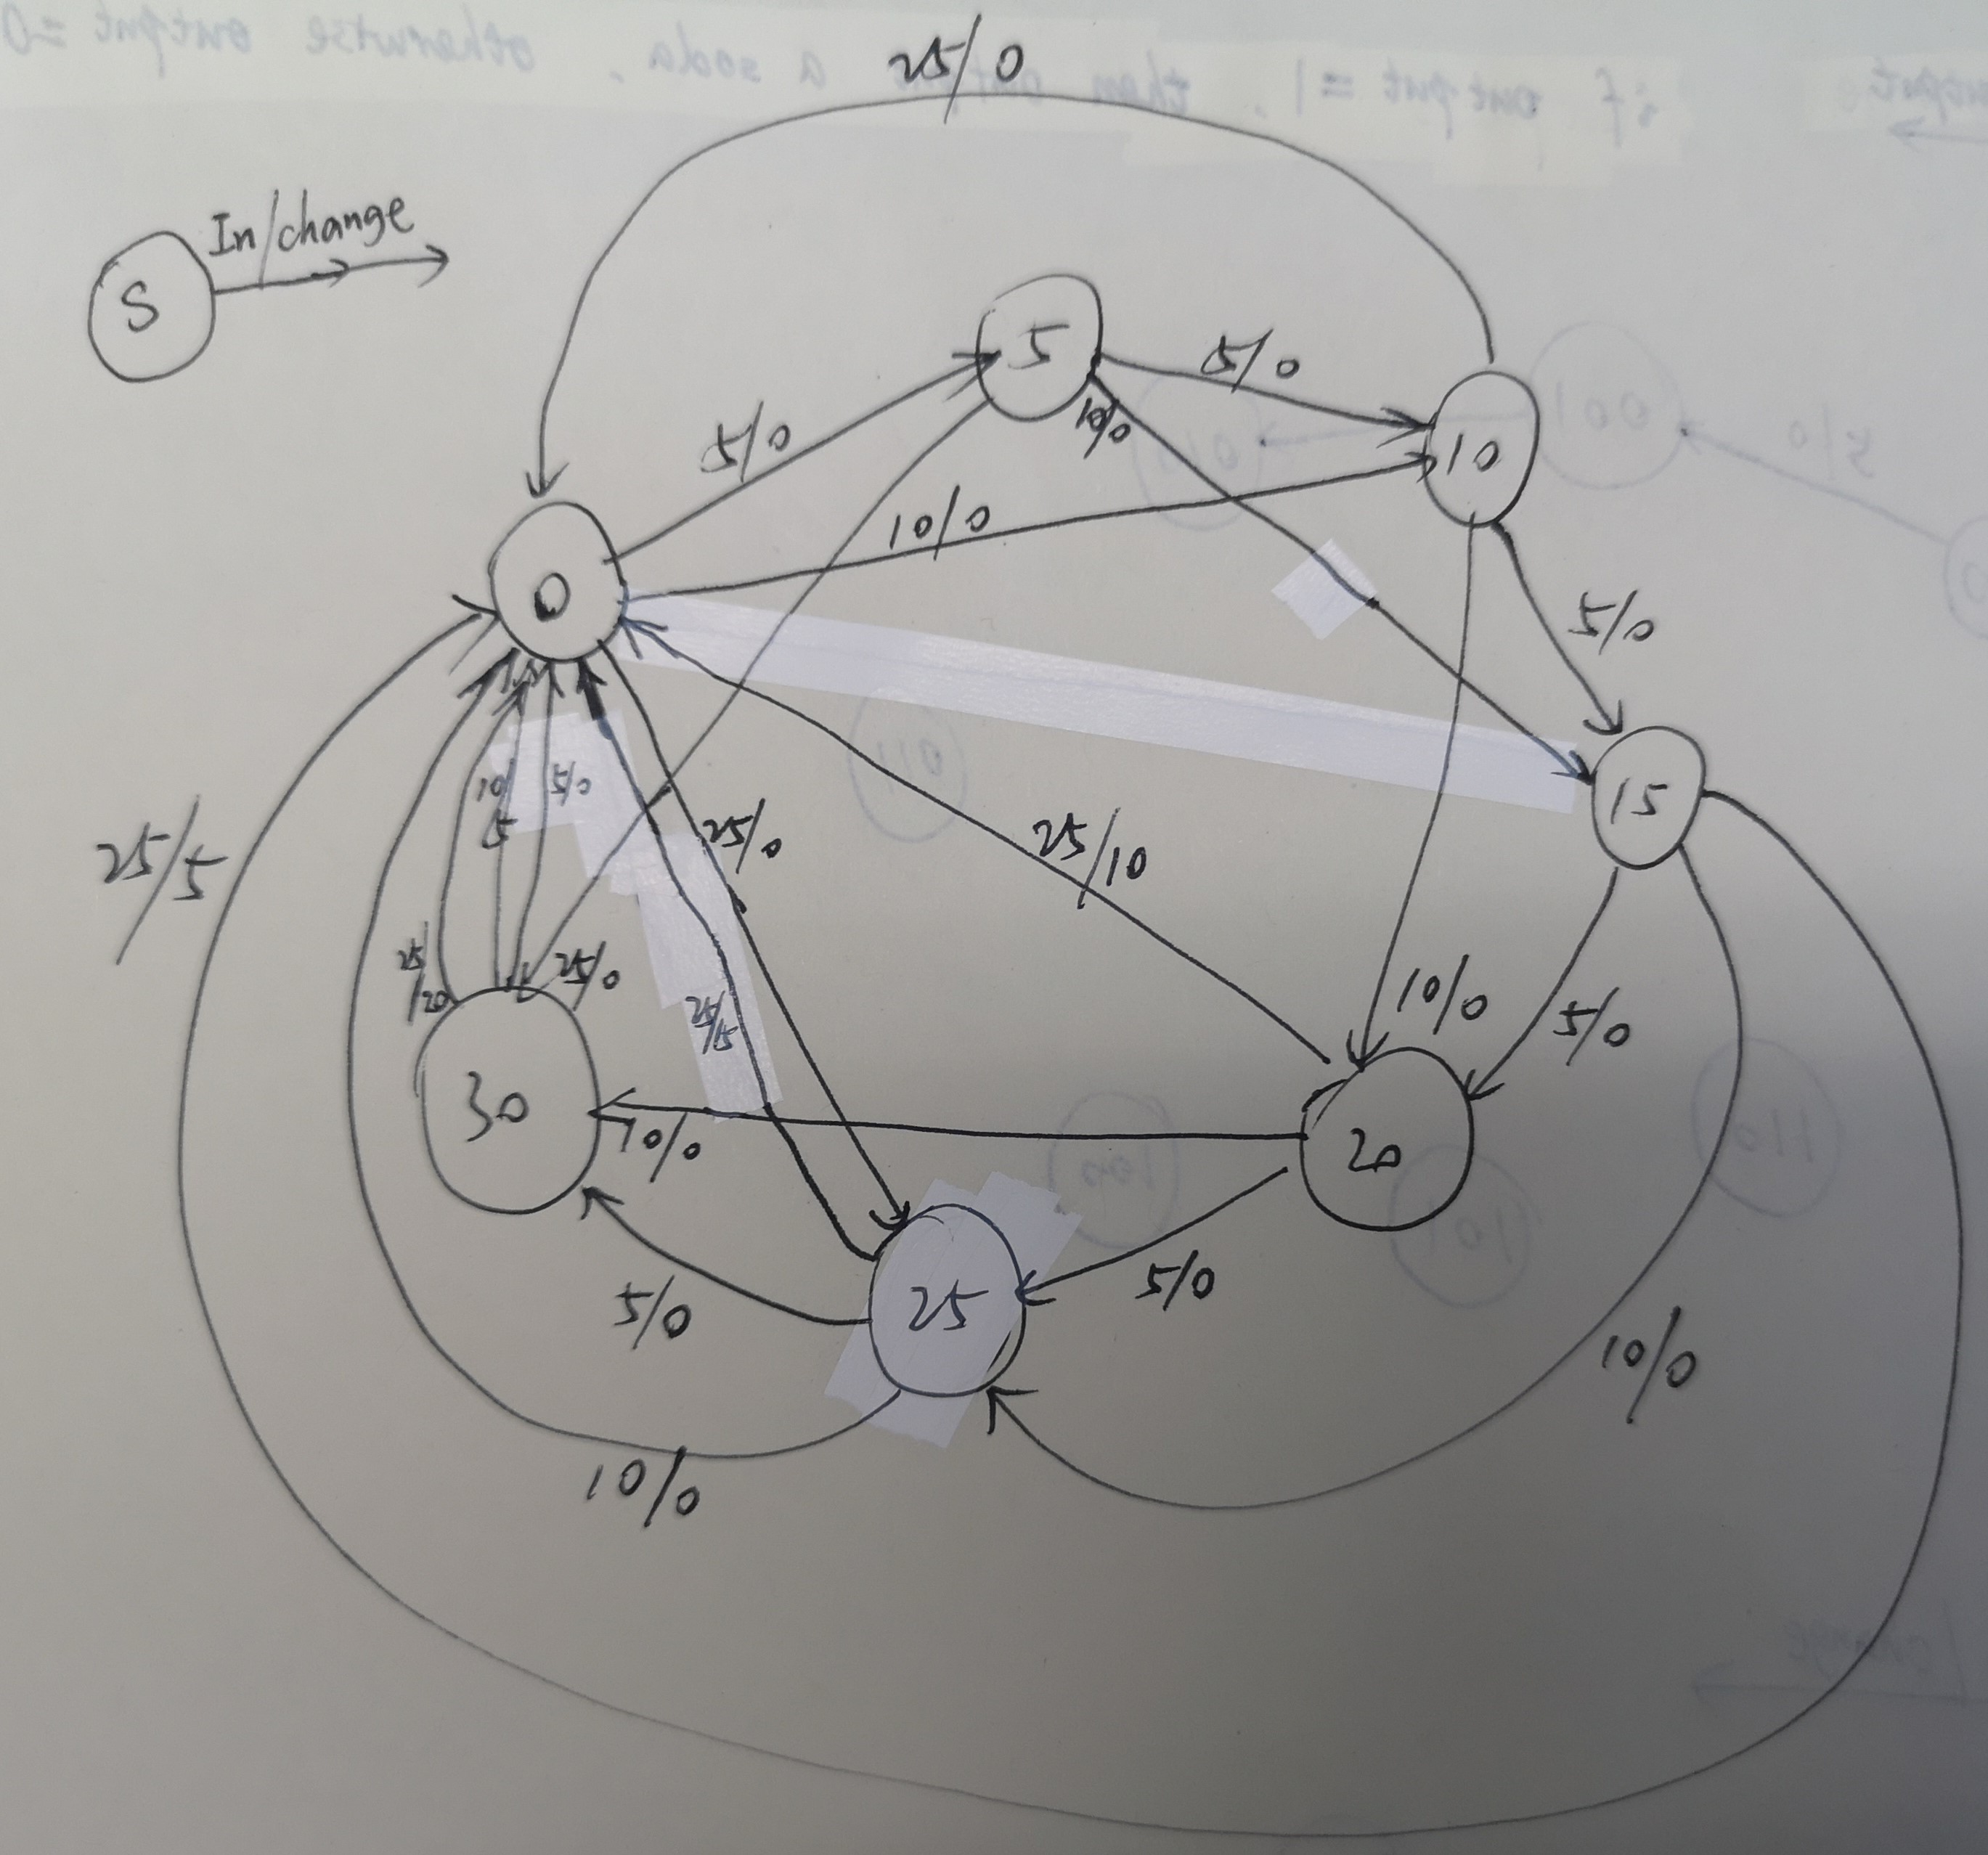
\includegraphics[width=1\linewidth]{5.jpg}
		\label{5}
	\end{figure}

	\section{\textcolor{red}{PAY ATTENTION TO THIS}}
	
	Using "-" to represent the state haven't been changed.
	\begin{table}[H]
		%\scriptsize
		\begin{tabular}{|c|c|c|c|c|c|c|c|}
			\hline 
			& PC & IR & MAR & MDR & R0 & R1 & R2\\ 
			\hline 
			Fetch & x3004 & x62BE & x3003 & x62BE & x3000 & x3000 & x3002 \\ 
			\hline 
			Decode & - & - & - & - & - & - & - \\ 
			\hline 
			Evaluate Address & - & - & - & - & - & - & - \\
			\hline 
			Fetch Operands & - & - & x3000 & x62BF & - & - & - \\ 
			\hline 
			Execute & - & - & - & - & - & - & - \\ 
			\hline 
			Store Result & - & - & - & - & - & x62BF & - \\ 
			\hline 
		\end{tabular} 
	\end{table} 

	\section{}
	\subsection*{a}
	$\lceil log_{2}(1151)\rceil=\underline{11\ bits}$.
	\subsection*{b}
	$\lceil log_{2}(40)\rceil=\underline{6\ bits}$.
	\subsection*{c}
	$32-11-6\times 3=\underline{3\ bits}$.
	
	\section{}
	\begin{lstlisting}[language=C]
	0101 000 000 1 00000	;AND R0, R0, #0
	1001 010 001 111111	;NOT R2, R1
	0001 010 010 1 00001	;ADD R2, R2, #1
	0001 010 010 000 011	;ADD R2, R2, R3
	0000 101 000000001	;BRnp
	0001 000 000 1 00001	;ADD R0, R0, #1
	1111 0000 0010 0101	;HALT
	\end{lstlisting}
	
	\section{}
	if R2 < R1, R4 = 0, otherwise, R4 = 1.
	
	
	
		
	
	

	
\end{document}